\chapter[Random Variables]{Random Variables}
\section{Random Variables: Examples and Definitions}
In practical applications we are typically interested in numerical features associated to an outcome of an experiment. 




These questions provide answers to very specific numeric/quantitative features of the student. 


Intuitively, a random variable measures a specific quantitative feature of the sample space outcome. Here is a schematic to consider: 
\begin{center}
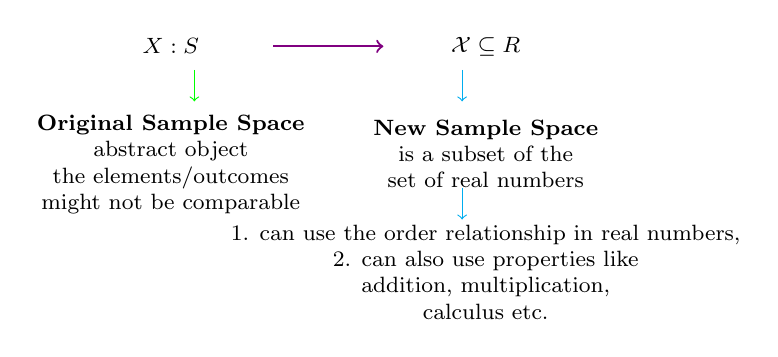
\begin{tikzpicture}
\tikzset{every node/.style={font=\footnotesize}}

% Function arrow and labels
\node at (-1.5, 0) (domain) {$X : S$};
\node at (2.5, 0) (codomain) {$\mathcal{X} \subseteq \mathbb{R}$};
\draw[->, thick, violet] (-0.2, 0) -- (1.2, 0);

% Left note
\node at (-1.5, -1.5) [align=center] {\textbf{Original Sample Space} \\ abstract object \\ the elements/outcomes \\ might not be comparable};

% Right note
\node at (2.5, -2.2) [align=center] {\textbf{New Sample Space} \\ is a subset of the \\ set of real numbers \\ \\ 1. can use the order relationship in real numbers, \\ 2. can also use properties like \\ addition, multiplication, \\ calculus etc.};

% Braces

% Arrows from notes to labels
\draw[->,green] (-1.2, -0.3) -- (-1.2, -0.7);
\draw[->,cyan] (2.2, -0.3) -- (2.2, -0.7);
\draw[->,cyan] (2.2, -1.8) -- (2.2, -2.2);

\end{tikzpicture}
\end{center}





%%%%%%%%%%%%%%%%%%%% Example: toss a coin three times %%%%%%%%%%%%%%%%




%%%%%%%%%%%%%%%%%%%%%%%%% end of example %%%%%%%%%%%%%%






%%%%% Example: Toss a coin once 





It is possible to classify all functions that can arise as cumulative distribution functions of random variable as follows:



\section{Discrete Random Variables}




It is easy to observe that the only points where $p_X$ can be non-zero are the values, $\mathcal{X}$, that $X$ can take. 




\section{Continuous Random Variables}









